% Following magic comments allow for compilation of root file
% !TEX root = ../../../../temp_manuscript.tex

\chapter{Introduction}
\glsresetall
\section{Glioma}

When cells reproduce, genetic changes can occur that result in the cells starting to grow uncontrollably.
This uncontrollable growth of new cells is commonly known as cancer.
When the cancerous cells clump together, the single mass that they form is called a tumour.
Tumours can originate from and occur almost everywhere in the human body, and the location where the tumour occurs is not always the same as the location from which the cancerous cells originate.
When the cancerous cells form a tumour in the location from which they originate, the tumour is called a primary tumour.
Hence, primary brain tumours are tumours located in the brain that are formed by cells that mutated from (healthy) brain cells.

Since different types of brain cells exist, the cancerous cells can have mutated from these different cells.
Therefore, primary brain tumours are categorized by the type of brain cells from which they mutated, with gliomas being the most prevalent \autocite{leece2017indicence}.
Gliomas are tumours which cancerous cells mutated from glial cells, which play a supporting role in the central nervous system and are the most abundant cell type in the brain \autocite{jakel2017glial}.
Although gliomas have a low incidence compared to other cancers, around \per{1.7} globally \autocite{leece2017indicence}, they are quite lethal with a median survival of around ten months \autocite{hess2004gliomaincidence}.

\section{Categorization of glioma}
Historically gliomas were categorized based solely on their histopathological appearance, the appearance of the tumour cells under a microscope.
Up to 2016, the \gls{WHO} recognized four different types of glioma: astrocytoma, oligoastrocytoma, oligodendroglioma, and glioblastoma (also known as \gls{GBM}).
This classification depended on the type of glial cells that were visible in the tumour tissue \autocite{louis2007who}.
Classifying glioma based on their glial cell type is often called typing.
In addition to glioma typing, tumours were assigned a grade to indicate their aggressiveness, this process is referred to as grading.
The grade was either II, III, or IV, with a grade IV glioma being the most aggressive.
Although grade I glioma exist, these are regarded as benign and as such are excluded from further consideration.
Grade II and grade III glioma are often referred to as \gls{LGG} and grade IV glioma are referred to as \gls{HGG}.
There is some relation between the type and grade of a glioma; glioblastoma are grade IV glioma, the most aggresive type, while astrocytoma, oligoastrocytoma, and oligodendroglioma are less aggressive and can be either grade II or grade III \footnote{Officially glioblastoma are grade IV astrocytoma, however in practice these are always referred to as gliobalastoma and astrocytoma mean to the grade II/III ones.}.

However, this categorization based on the typing and the grading of the tumour is suboptimal.
Firstly, the histopathological categorization and grading of the tumours are very observer dependent \autocite{mittler1996gradingreliability, vandenbent2010interobserver}.
Since the clinical decision making depended on the categorization, this observer dependency could lead to a inadequate treatment of the tumour \autocite{vandenbent2010interobserver}.
Secondly, within these categories, large differences between the survival of patients existed, suggesting a different underlying mechanic at play that determines the aggressiveness of the tumour \autocite{dubbink2015molecular}.
For example, some grade III glioma showed survival rates more characteristic of grade IV glioma than other grade III glioma.
It was found that this difference can be explained by the genetic features of the tumour \autocite{dubbink2015molecular,eckel2015gliomagroups}.
Therefore, in 2016 the \gls{WHO} updated the categorization of glioma to include these genetic features and depend less on the histopathology alone \cite{louis20162016}.
This update led to better patient stratification and more objective categorization of glioma \autocite{molinaro2019geneticepidemiology}.

In the updated guidelines the tumour typing has become less relevant.
The histopathology now only needs to distinguish astrocytoma, oligoastrocytoma, oligodendroglioma (\gls{LGG}) on the one hand and glioblastoma (\gls{HGG}) on the other hand.
This greatly reduces the observer variability as most variability was observed in distinguishing between astrocytoma, oligoastrocytoma, and oligodendroglioma \autocite{mittler1996gradingreliability}.
Further categorization of the glioma is now based on two genetic features:  the \gls{IDH} mutation and \acl{1p19qcotion}.
These are two genetic features that occur at specific parts of the genome, but only occurs in the genome of the tumour and not in the genome of the healthy tissue.
When the \gls{IDH} gene is normal (the same as the \gls{IDH} gene of the healthy tissue) the tumour is referred to as \gls{IDH} wildtype.
If the \gls{IDH} gene is mutated from the normal gene the tumour is a \gls{IDH} mutated tumour.
The same holds for the \acl{1p19qcotion}: if it is the same as the original gene it is \acl{1p19qint}, if it mutated from the original it is \acl{1p19qcodel}.

Within the \gls{LGG} (what was previously astrocytoma, oligoastrocytoma, and oligodendroglioma), the following categories now exist:
\begin{itemize}
    \item Diffuse astrocytoma, \gls{IDH} wildtype
    \item Diffuse astrocytoma, \gls{IDH} mutated
    \item Oligodendroglioma, \gls{IDH} mutated and 1p/19q codeleted
\end{itemize}
No category exists for \gls{IDH} wildtype, 1p/19q co-deleted glioma since as it was found that all 1p/19q co-deleted tumours are also IDH mutated \autocite{labussi20101p19qcodeletedIDH}.
Although the terms astrocytoma and oligodendroglioma are still used in the updated guidelines, they no longer carry the same meaning as before, since their categorization is no longer based on the glial cell type but instead on the genetic features.
The oligodendroglioma group has the best prognosis among the \gls{LGG}, with the diffuse astrocytoma IDH wildtype showing the worst prognosis.
Due to the aggressiveness of IDH wildtype astrocytoma, it is even suggested that these are actually misclassified glioblastoma \autocite{hartmann2010IDH1gbm, brat2018IMPACT}.
An overview of the \gls{WHO} 2016 guidelines and their relation to the previous guidelines is presented in \cref{fig:intro_glioma_categorization}.


\begin{figure}[hbt]
    \resizebox{0.8\textwidth}{!}{\subimport{Figures/}{WHO_2016_flowchart.pgf}}
    \centering
    \caption{The WHO 2016 categorizaton of glioma.}\label{fig:intro_glioma_categorization}
\end{figure}

The \gls{WHO} 2016 guidelines also categorize glioblastoma based on the \gls{IDH} mutation status, with \gls{IDH} mutated glioblastoma having a better prognosis than \gls{IDH} wildtype glioblastoma.
Although the guidelines currently only include the \gls{IDH} mutations status, there is another genetic feature that plays an important role in glioblastoma: \gls{MGMT} methylation.
\gls{MGMT} methylation is an important genetic features, where patients with \gls{MGMT} methylated tumours survive longer than patients with \gls{MGMT} unmethylated tumours \autocite{martinez2007MGMT, gessler2018MGMT, weller2009molecularGBM}.
Thus, although not officially part of the most recent \gls{WHO}, guidelines the \gls{MGMT} methylation status is now often relevant in the clinical decision making \cite{molinaro2019geneticepidemiology}.

Not only is there a difference in the tumour aggressiveness depending on their genetic features, but tumours also respond differently to certain treatments based on their genetic features.
For example \gls{IDH} mutated glioma respond better to radiotherapy than \gls{IDH} wildtype glioma \autocite{juratli2015IDHtreatment}, and the 1p19q co-deletion status and MGMT methylation status might be predictors of the sensitivity to chemotherapy \autocite{idbaih2007markersresponse}.
Thus, it is important to know the genetic features of a glioma, both for the prognosis of the patient and for the clinical decision making.

In current clinical practice, the genetic features are determined either from a biopsy, or a resection.
In the case of a biopsy, a small part of the tumour is removed for analysis to decide on the further treatment of the tumour.
Thus, biopsies are not part of the treatment but are merely used to decide on further treatment options.
Resection is part of the treatment process, and involves surgically removing as much of the tumour as possible.
Part of the removed tumour can then be used for the genetic and histopathological analysis to decide on follow-up treatments.
Taking a biopsy or resecting the tumour requires intrusive surgery, which can negatively impact the patient.
Therefore, it would be beneficial if the genetic features of a glioma can be determined without the need for a biopsy or resection.
This is especially relevant in the case of a biopsy since the sole purpose of the biopsy is to obtain tissue that can be analyzed to help the clinical decision making.

A non-invasive method to determine the genetic features of the tumour not only obviates the need for an intrusive surgical operation, but it can also provide relevant information earlier in the treatment process, which can aid in the clinical decision making.
In some cases, especially for IDH mutated, 1p/19q co-deleted glioma, it might be better to follow a watch-and-wait approach since leaving tumour untreated might have less of a negative impact than the potentially damaging effect of the treatment on the healthy tissue \autocite{vandenbent2012lggtreatment, welle2017EANO}.
Since \gls{MRI} is already part of the standard clinical pathway for glioma patients, it is the ideal candidate for a non-invasive way of identifying the genetic features of the tumour.

\section{MRI image analysis of glioma}

\gls{MRI} is an imaging technique that uses the magnetic properties of protons, one of three elementary particles that form an atom, to create an image.
Although protons appear in all atoms, hydrogen atoms are of particular interest because they consist of a single proton.
Furthermore, a water molecule contain two hydrogen atoms and since the majority of the human body consists of water, hydrogen atoms (and thus protons) are abundant in the human body, especially in soft tissue.
An \gls{MRI} scanner manipulates the protons to form an image and can even manipulate them in different ways to obtain different imaging contrasts.

\gls{MRI} is routinely used in clinical care to distinguish between healthy and diseased tissue.
Shortly after the first introduction of \gls{MRI}, it was proposed that the method could be used to identify tumours \autocite{damadian1971tumour}.
After some improvements, the technique was first applied to the brain in 1980 \autocite{holland1980brain}, and in the same year MRI was first used to investigate a brain tumour \autocite{hawkes1980NMRbrain}.
Since then the quality of \gls{MRI} scans has vastly improved and different \gls{MRI} techniques have been developed that can image different tissue characteristics.
\cref{fig:intro_MR_example} shows some of the currently most popular imaging sequences, although many more exist.
In these scans the tumour can clearly be seen, which gives the clinician important information in a non-invasive way with minimal risk for the patient.
Therefore, \gls{MRI} is part of the standard-of-care for brain tumour diagnosis and treatment decisions.

\begin{figure}[hbt]
    \centering
    \begin{subfigure}[b]{0.45\textwidth}
        \centering
        \includegraphics[width=\textwidth]{example-image-a}
        \caption{First scan of a human glioma}\label{fig:intro_MR_first}
    \end{subfigure}
    \begin{subfigure}[b]{0.45\textwidth}
        \centering
        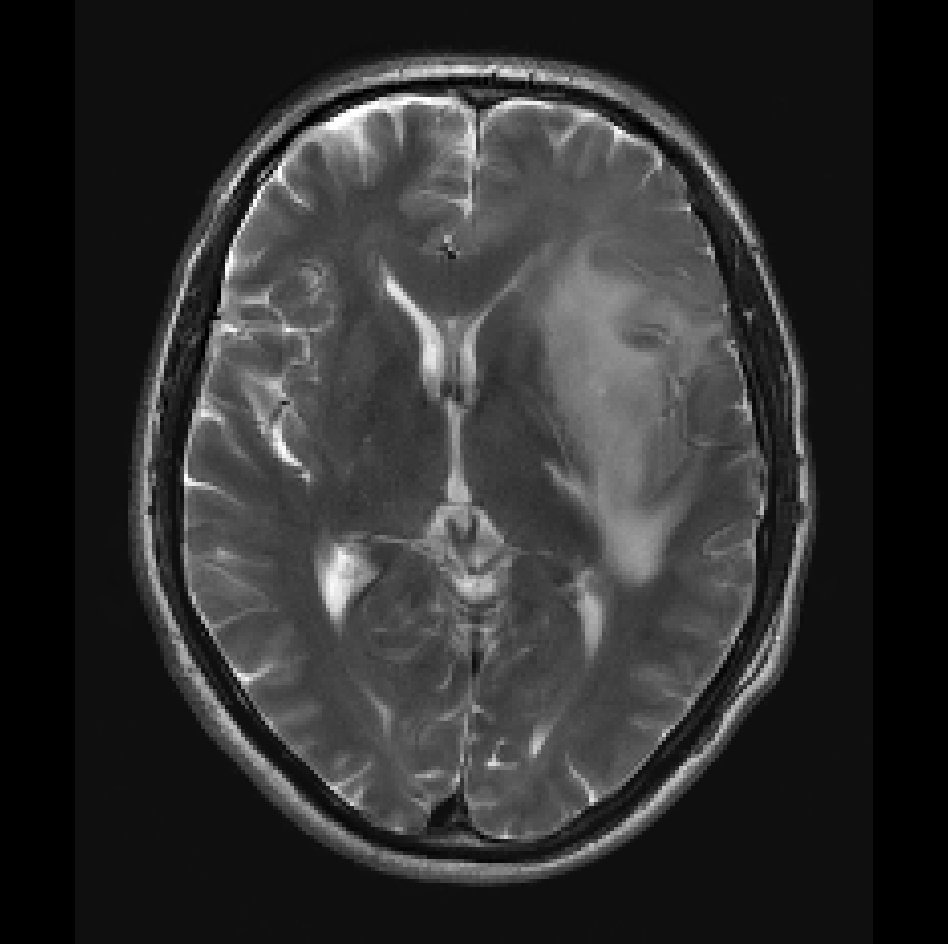
\includegraphics[width=\textwidth]{Figures/T2_LGG.png}
        \caption{Modern glioma scan}\label{fig:intro_MR_modern}
    \end{subfigure}
    \caption{\acrshort{MRI} scan of a glioma from 1980 and a recent \acrshort{MR} scan, showing the large improvement over time. On the modern scan the glioma can easily be identified}\label{fig:intro_MR_example}
\end{figure}

\gls{MRI} scans are already routinely being used to get a first indication of the aggressiveness of the tumour, mainly for tumour grading \autocite{upadhyay2011MRIevaluation}.
With the increasing importance of genetic features of the tumours, research has focused on identifying imaging features that correlate with the genetic features of a tumour \autocite{patel2017mismatch, smits2016imaging}.
These imaging features that correlate with an underlying physiological aspect, in this case the genetic features, are called imaging biomarkers.
The presence of these biomarkers proves the potential of \gls{MRI} as a non-i nvasive alternative to tumour biopsy and resection.
However, their use in clinical practice is still limited.

The widespread use of biomarkers for the genetic features of a glioma is faced by a few problems.
Firstly, the biomarkers have to be relatively simple, because clinicians need to be able to quickly and easily extract them from the scans.
For example, most current clinically used biomarkers rely on 2D measurements (whereas the tumour is of course 3D), or only consider a single point or small area of the tumour instead of the whole tumour.
As a result the information included in these biomarkers is limited, whereas using more information could lead to a better correlation with the physiological aspect of interest.
Secondly, \gls{MRI} is a qualitative and not a quantitative measurement, meaning that only the contrast of the scan and not its absolute value contain information \footnote{This is similar to food; it is easy to say that chocolate tastes better than brussel sprouts, but one cannot say that chocolate tastes 5 \say{taste units} and brussel sprouts tastes 1 \say{taste unit}.}.
Because of this scans from the same patient from two different \gls{MRI} machines might have a similar visual appearance, but can result in different values for the same biomarker.
This complicates the use of these biomarkers as it is not possible to use the absolute value of these biomarkers.
Thirdly, partly due to the previous point, the biomarkers are often vaguely defined.
Instead of defining a quantitative biomarker, qualitative biomarkers are used based on the interpretation of the visual appearance of the tumour.
For example, a score can be assigned to how aggressive the tumour looks.
This leads to biomarkers that are, similar to the typing and grading that was done before, observer dependent.
Lastly, only a limited set of biomarkers is extracted and used for the correlation with the clinical outcome.
The method to correlates the biomarkers with the clinical outcome has to be simple to make it viable for the clinical experts to use.
Thus, although some promising biomarkers have been found there is a need for new biomarkers and new methods that can include more information from the \gls{MR} scan, are more objective, more consistent and, most importantly, do not put an additional burden on the clinicians.


\section{Goals of this thesis}

This thesis has three main goals;

\begin{enumerate}
\item Find more objective biomarkers for the genetic features of glioma, that experts can easily use
\item Provide tools and data to make research into new biomarkers easier
\item Provide information that is normally obtained from invasive procedures from \gls{MRI} scans
\end{enumerate}

To achieve these goals I focus on automated, computational methods.
Automated methods can carry out certain complex tasks more easily than humans, and do so in an objective, consistent way \footnote{Not all automated methods are necessarily consistent, some might contain a random element (purposefully or not). In this case the potential inconstancy of the automated methods is negligible compared to the inconstancy of humans.}.

We define two types of automated methods: algorithmic methods and machine learning methods.
Algorithmic methods are methods where the process of determining an output from its inputs is explicitly defined by a human.
For example, the addition operator ($+$) is an algorithmic method, since we can now give two inputs and now exactly what our method will do with them.
In this way we can create methods that can perform certain tasks very quickly which might be complex to do manually.
For example, these methods can very easily determine the 3D measurements of a tumour.
In this way it is possible to extract more complicated biomarkers, without any observer dependency.

On the other hand are machine learning methods, which have become popular in recent years.
Machine learning methods are methods where the process of computing an output form its outputs is not explicitly defined, but is left up to the method to figure out.
These methods do so by taking (a large amount of) data, and try to find patterns in the input data that can be used to correlate it with the output data.
For example, a machine learning method could be given a long list of two inputs and one output, where the output is the addition of the two inputs.
It is then up to the machine learning method to figure out that it needs to sum to two inputs to get the correct output.
In this way machine learning methods can learn relationships that were not yet known by clinical experts, making them a very versatile tool.

Using (a combination of) these methods allows us to achieve the goals outlined above and can solve the problems currently faced when using biomarkers in the clinic.
By taking the human aspect out of the extraction of biomarkers, the biomarkers can be more complicated and are not observer-dependent.
Furthermore, these automated methods can very fast, alleviating some of the burden placed on clinical experts.
When implemented properly these methods are also widely applicable and do not require additional clinical expertise.
By using the strengths of automated methods to replace the current weaknesses of the manual methods, we can provide more and better information and allow the strength of clinical experts to shine as well; the abstract process of decision making when presented with the relevant clinical information.

\section{Thesis outline}

\cref{chap:radiomics} provides an in-depth introduction of machine learning methods, introduces common terminology, and discusses some of the issues that can be encountered in machine learning research.

In \cref{chap:LGGLocation} I use automated methods to find new biomarkers for \gls{LGG}, specifically looking for a relationship between the location of the glioma in the brain and its genetic features.
The same methods are then used to establish a relationship between the genetic features of \gls{HGG} and their location in \cref{chap:HGGLocation}, now considering genetic features that are relevant for \gls{HGG}.

In \cref{chap:LGG1p19q} I further investigate potential biomarkers in \gls{LGG}, specifically for the 1p/19q co-deletion status.
These biomarkers are automatically extracted from the \gls{MRI} scans, to include more complex information than manually viable biomarkers.
I then use a machine learning method to link the biomarkers with the 1p/19q co-deletion status and compare the performance of this method with the performance of clinical experts.

Since machine learning methods require (often large amounts of) data, in \cref{chap:DDS} I developed a method that automatically sorts large amounts of \gls{MRI} scans.
In this way it is possible to quickly go from a data from the clinical practice to data that can be used for research.

Finally, in \cref{chap:discussion} I discuss the results from this thesis and explore possible future research directions.
I also provide an overview of the potential clinical applications that the methods developed in this thesis and other automated methods can have in the image analysis of glioma.

